
\section{The Lusternik-Schnirelmann category}

For topological spaces the criteria of having trivial cup products is quite strong. Say 
we have a path-connected topological space $X$. It has zeroth cohomology $H^0(X;K)\cong K$. 
Hence the requirement to have trivial cup product reduces to requiring $H^i(X;K)=0$ for 
$i>0$, which is really limiting. One solution to this is to look at reduced cohomology. 

\begin{definition}
    Let $X$ be a topological space and $C^\ast(X;K)$ its cochain complex (treated here as a 
    dg-algebra). We define its augmented cochain dg-algebra, denoted 
    $\widetilde{C}^\ast(X;K)$, by adding a copy of the ground field $K$ injectively farthest 
    to the left, i.e.
    \begin{equation*}
        \cdots \longrightarrow 0 \longrightarrow K \overset{\epsilon}\longrightarrow 
        C^0(X;K)\longrightarrow C^1(X;K) \longrightarrow \cdots \longrightarrow C^n(X;K) 
        \longrightarrow \cdots  
    \end{equation*}
\end{definition} 

The cohomology algebra of the augmented cochain complex is called the reduced cohomology 
algebra of $X$ and is denoted $\widetilde{H}^\ast(X;K)$. If the space $X$ is connected, 
then $\widetilde{H}^0(X;K)=0$, meaning that we have completely removed the problem 
described above. 

Spaces with trivial cup product are not in abundance -- even in reduced cohomology -- 
but examples include the spheres and more generally a suspended space. There are ways to 
make sure that a space has a trivial cup product and one of these is using the 
Lusternik-Schnirelmann category. 

\begin{definition}
    Let $X$ be a topological space. The Lusternik-Schnirelmann category of $X$, denoted 
    $\text{cat}_{LS}(X)$, is the least integer $n$ such that there is a covering of $X$ 
    by $n+1$ open subsets $U_i$ that are all contractible in $X$, i.e. their inclusion 
    into $X$ is null-homotopic.    
\end{definition}

This invariant was originally developed in \cite{lscat} as an invariant on manifolds to be 
a lower bound for the number of critical points any real valued function on it could have. 
It has since become a useful – but very difficult to calculate – invariant of topological 
spaces. 

Recall that the cup-length of a topological space 
$X$, denoted $\text{cl}(X)$ is the largest integer $n$ such that a chain 
$[x_1]\cup \cdots \cup [x_n]$ of cohomology classes with $\deg|x_i|\geq 1$ is non-zero. 
We have the following fundamental relation between the cup length and the 
Lusternik-Schnirelmann category of $X$.

\begin{lemma}[\cite{lscategorybook}]
    Let $X$ be a topological space. Then the cup length of $X$ is a lower bound for its 
    Lusternik-Schnirelmann category, i.e. $\text{cl}(X)\leq \text{cat}_{LS}(X)$.    
\end{lemma}

Thus, choosing spaces with $\text{cat}_{LS}(X) = 1$ means we have trivial product on 
reduced cohomology. Examples of such spaces are again the suspended spaces, as they are 
the union of two cones. The last thing we need to know is whether spaces with 
Lusternik-Schnirelmann category $1$ admit any non-vanishing Massey  $n$-products. Luckily, 
by Rudyak we know that they dont.

\begin{theorem}[\cite{Rudyak}]
    \label{thm:rudyak}
    Let $X$ be a topological space with $\text{cat}_{LS}(X)\leq 1$ and 
    $x_1, \ldots, x_n \in \widetilde{H}^\ast(X;K)$. If the Massey $n$-product 
    $\langle x_1, \ldots, x_n\rangle$ is defined then 
    $\langle x_1, \ldots, x_n\rangle = 0$.    
\end{theorem}

We call spaces with formal reduced cochain algebras reduced formal spaces. This means now
that spaces with Lusternik-Schnirelmann category $1$ are reduced formal by 
\cref{thm:rudyak} and \cref{thm:1}. 

\begin{corollary}
    \label{cor:reduced_formal}
    Let $X$ be a topological space with $\text{cat}_{LS}(X)\leq 1$. Then 
    $\widetilde{C}^\ast(X;K)$ is a formal dg-algebra. 
\end{corollary}

We still have to deal with the degree $0$ cochains in order to say that a space $X$ with
$\text{cat}_{LS}(X)\leq 1$ is formal and not just reduced formal. To do this we must 
construct the neccesary span of dg-quasi-isomorphism.

\begin{theorem}
    \label{thm:reduced_formal_formal}
    Any reduced formal topological space $X$ is formal.     
\end{theorem}

\begin{proof}
    Since $X$ is reduced formal we know that there is a span of dg-quasi-isomorphisms 
    $$\widetilde{H}^\ast(X;K)\longleftarrow B \longrightarrow \widetilde{C}^\ast(X;K)$$ for some 
    dg-algebra $B$:

    \begin{center}
        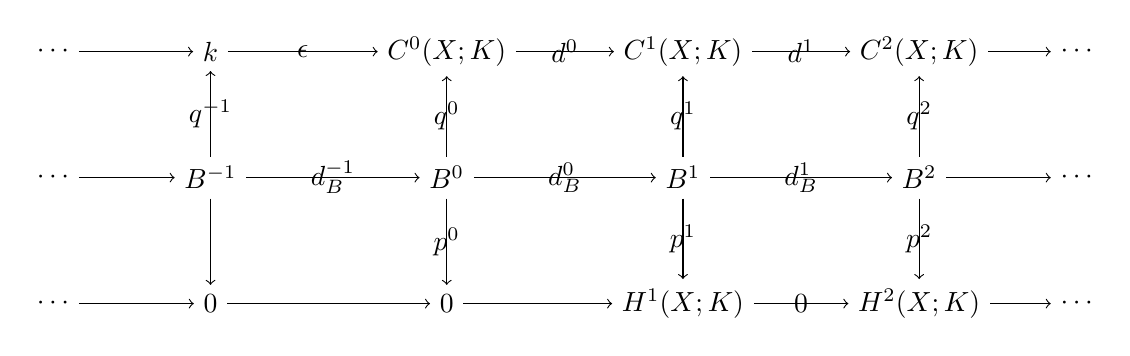
\begin{tikzpicture}
            \node (1) {$k$};
            \node (2) [node distance=3cm, right of=1] {$C^0(X;K)$};
            \node (3) [node distance=3cm, right of=2] {$C^1(X;K)$};
            \node (4) [node distance=3cm, right of=3] {$C^2(X;K)$};
            
            \node (5) [node distance=1.6cm, below of=1] {$B^{-1}$};
            \node (6) [node distance=3cm, right of=5] {$B^0$};
            \node (7) [node distance=3cm, right of=6] {$B^1$};
            \node (8) [node distance=3cm, right of=7] {$B^2$};
            
            \node (9) [node distance=1.6cm, below of=5] {$0$};
            \node (10) [node distance=3cm, right of=9] {$0$};
            \node (11) [node distance=3cm, right of=10] {$H^1(X;K)$};
            \node (12) [node distance=3cm, right of=11] {$H^2(X;K)$};
            
            \node (13) [node distance=2cm, left of=1] {$\cdots$};
            \node (14) [node distance=2cm, left of=5] {$\cdots$};
            \node (15) [node distance=2cm, left of=9] {$\cdots$};
            \node (16) [node distance=2cm, right of=4] {$\cdots$};
            \node (17) [node distance=2cm, right of=8] {$\cdots$};
            \node (18) [node distance=2cm, right of=12] {$\cdots$};
            
            \draw [-to] (13) to node {} (1);
            \draw [-to] (14) to node {} (5);
            \draw [-to] (15) to node {} (9);
            \draw [-to] (4) to node {} (16);
            \draw [-to] (8) to node {} (17);
            \draw [-to] (12) to node {} (18);
            
            \draw [-to] (1) to node {$\epsilon$} (2);
            \draw [-to] (2) to node {$d^0$} (3);
            \draw [-to] (3) to node {$d^1$} (4);
            
            \draw [-to] (5) to node {$d^{-1}_B$} (6);
            \draw [-to] (6) to node {$d^0_B$} (7);
            \draw [-to] (7) to node {$d^1_B$} (8);
            
            \draw [-to] (9) to node {} (10);
            \draw [-to] (10) to node {} (11);
            \draw [-to] (11) to node {$0$} (12);
            
            \draw [-to] (5) to node {$q^{-1}$} (1);
            \draw [-to] (5) to node {} (9);
            
            \draw [-to] (6) to node {$q^0$} (2);
            \draw [-to] (6) to node [swap]{$p^0$} (10);
            
            \draw [-to] (7) to node {$q^1$} (3);
            \draw [-to] (7) to node [swap]{$p^1$} (11);
            
            \draw [-to] (8) to node {$q^2$} (4);
            \draw [-to] (8) to node [swap]{$p^2$} (12);
        \end{tikzpicture}
        \end{center}

    By removing the copy of $k$ from the augmented cochain complex, we can insert
    a copy of $k$ as $H^0(X;K)$ and form a new span of dg-quasi-isomorphisms:

    \begin{center}
        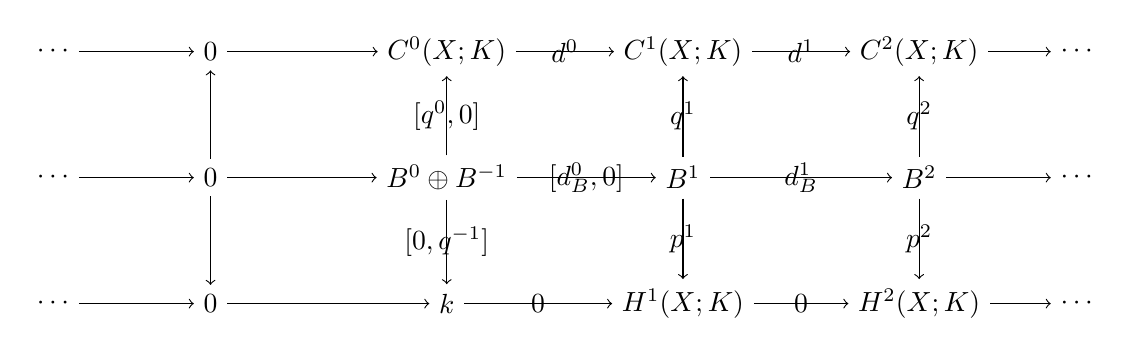
\begin{tikzpicture}
            \node (1) {$0$};
            \node (2) [node distance=3cm, right of=1] {$C^0(X;K)$};
            \node (3) [node distance=3cm, right of=2] {$C^1(X;K)$};
            \node (4) [node distance=3cm, right of=3] {$C^2(X;K)$};
            
            \node (5) [node distance=1.6cm, below of=1] {$0$};
            \node (6) [node distance=3cm, right of=5] {$B^0\oplus B^{-1}$};
            \node (7) [node distance=3cm, right of=6] {$B^1$};
            \node (8) [node distance=3cm, right of=7] {$B^2$};
            
            \node (9) [node distance=1.6cm, below of=5] {$0$};
            \node (10) [node distance=3cm, right of=9] {$k$};
            \node (11) [node distance=3cm, right of=10] {$H^1(X;K)$};
            \node (12) [node distance=3cm, right of=11] {$H^2(X;K)$};
            
            \node (13) [node distance=2cm, left of=1] {$\cdots$};
            \node (14) [node distance=2cm, left of=5] {$\cdots$};
            \node (15) [node distance=2cm, left of=9] {$\cdots$};
            \node (16) [node distance=2cm, right of=4] {$\cdots$};
            \node (17) [node distance=2cm, right of=8] {$\cdots$};
            \node (18) [node distance=2cm, right of=12] {$\cdots$};
            
            \draw [-to] (13) to node {} (1);
            \draw [-to] (14) to node {} (5);
            \draw [-to] (15) to node {} (9);
            \draw [-to] (4) to node {} (16);
            \draw [-to] (8) to node {} (17);
            \draw [-to] (12) to node {} (18);
            
            \draw [-to] (1) to node {} (2);
            \draw [-to] (2) to node {$d^0$} (3);
            \draw [-to] (3) to node {$d^1$} (4);
            
            \draw [-to] (5) to node {} (6);
            \draw [-to] (6) to node {$[d^0_B, 0]$} (7);
            \draw [-to] (7) to node {$d^1_B$} (8);
            
            \draw [-to] (9) to node {} (10);
            \draw [-to] (10) to node {$0$} (11);
            \draw [-to] (11) to node {$0$} (12);
            
            \draw [-to] (5) to node {} (1);
            \draw [-to] (5) to node {} (9);
            
            \draw [-to] (6) to node {$[q^0, 0]$} (2);
            \draw [-to] (6) to node [swap]{$[0, q^{-1}]$} (10);
            
            \draw [-to] (7) to node {$q^1$} (3);
            \draw [-to] (7) to node [swap]{$p^1$} (11);
            
            \draw [-to] (8) to node {$q^2$} (4);
            \draw [-to] (8) to node [swap]{$p^2$} (12);
        \end{tikzpicture}
        \end{center}

    The squares in the diagram commutes due to the original squares commuting
    and the cohomologies also agree by construction. Thus we have a span of 
    dg-quasi-isomorphisms $$H^\ast(X;K)\longleftarrow B'\longrightarrow C^\ast(X;K),$$ 
    which means $X$ is formal. 
\end{proof}

We are now ready to conclude with our main result.
\begin{theorem}
    Let $X$ be a space with $\text{cat}_{LS}(X)\leq 1$. Then $X$ is formal.     
\end{theorem}

\begin{question}
    Are there any formal spaces with trivial cup product and Lusternik-Schnirelmann 
    category greater than $1$? 
\end{question}